Here, we are given a sentence $\mathcal{S}$ as a $N$-length sequence of tokens, $\mathcal{S} = \langle w_1, w_2 \ldots w_N \rangle$ and a span $\langle s, e\rangle$ where $s \in [1, N]$ is the \textit{start} index, $e \in [1, N]$ is the \textit{end} index. The goal is to output a label $t$ for the span such that $t \in \mathcal{T}$, where $\mathcal{T}$ is the set of all entity types.

This is modeled as the reverse of QA model for NER described in Section \ref{sec:span}. For every gold entity mention (E.g. \textit{United States}) in a training set sentence, \textit{Emily}[\texttt{PERSON}] \textit{lives in United States}[\texttt{LOCATION}], we form a sample input, \textit{Emily lives in United States. What is United States?} The sentence is fed to a BERT model where we do sequence classification. The pooled sequence embedding returned by BERT is fed to a fully connected layer and converted to a probability distribution over possible entity types. In this example, the model is expected to assign maximum probability to \texttt{LOCATION}. Figure \ref{fig:span_classification} shows our span classification setup.

\begin{figure}[h!]
    \centering
    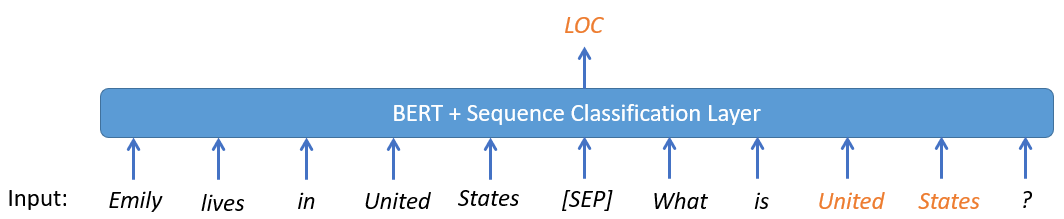
\includegraphics[width=\linewidth]{../thesis/span_classification}
    \caption{Span Classification Setup (colored tokens depict the entity mention in question with expected output entity label)}
    \label{fig:span_classification}
\end{figure}

